\documentclass[10pt]{article}
\usepackage{commands}


\begin{document}
\begin{tcolorbox}
  \begin{center}
  \begin{Large}
    \textbf{PHYS 500 (Quantum Mechanics I) Notes} \\
    \vspace{5pt}
  \end{Large}
  \begin{large}
        Rio Weil \\
\vspace{5pt}
    \emph{This document was typeset on \today}
  \end{large}
  \end{center}
\end{tcolorbox}

\begin{center}
  \textbf{Introduction:}

  This is a set of lecture notes taken from UBC's PHYS 500 (Graduate Quantum Mechanics I) course, taught by Dr.\ Ariel Zhinitsky. The course covers Angular momentum and spin, electromagnetic interactions, Time-independent perturbation theory, the WKB approximation, Time-dependent perturbation theory, the adiabatic approximation, and scattering. If any errors are found in the notes, feel free to email me at \href{mailto:ryoheiweil@phas.ubc.ca}{ryoheiweil@phas.ubc.ca}.

\end{center}
\addtocontents{toc}{\protect\hypertarget{toc}{}}
\tableofcontents

\newpage
\section{Angular Momentum}

\subsection{Units}
We set $\hbar = 1$ for this course (natural units), unless we are doing a numerical estimate of some quantity.

\subsection{Angular Momentum - Definitions}
Angular momentum operators obey the commutation relations:
\begin{equation}
    [L_i, L_j] = i\e_{ijk}L_k.
\end{equation}
Where $\e_{ijk}$ is the Levi-Cicata symbol, defined as:
\begin{equation}
    \e_{ijk} = \begin{cases}
        +1 & ijk \text{ is an even permutation of 123}
        \\ -1 & ijk \text{ is an odd permutation of 123}
        \\ 0 & \text{otherwise}
    \end{cases}
\end{equation}
We also follow the Einstein summation convention, where repeated indices are implicitly summed over. We also define the raising/lowering operators:
\begin{equation}
    L_{\pm} = L_x \pm iL_y
\end{equation}
and the total angular momentum:
\begin{equation}\label{eq-Lsquared}
    \v{L}^2 = L_x^2 + L_y^2 + L_z^2.
\end{equation}
It can be easily verified that:
\begin{equation}
    [\v{L}^2, L_i] = 0
\end{equation}
and that:
\begin{equation}
    [L_z, L_+] = [L_z, L_x + iL_y] = +L_+
\end{equation}
\begin{equation}
    [L_z, L_-] = -L_-
\end{equation}
\begin{equation}
    [\v{L}^2, L_\pm] = 0
\end{equation}
Note that while $L_i$ are Hermitian operators (they are observables), the $L_\pm$ are not (this can be verified by the definition of the Hermitian conjugate). However this does not mean that it is not useful. Now, we ask, what is the physical meaning of:
\begin{equation}
    [\v{L}^2, L_z] = 0
\end{equation}
The answer is that we can know/measure $\v{L}^2$ and $L_z$ simultaneously. Next, what is the meaning of:
\begin{equation}
    [\v{L}^2, L_\pm] = 0
\end{equation}
This means that if we apply $L_{\pm}$ to an eigenstate of $\v{L}^2$, we do not change the eigenstate. Now, what is the physical meaning of:
\begin{equation}
    [L_z, L_+] = L_+?
\end{equation} 
It tells us that $L_+$ is a raising operator for $L_z$; it increments the eigenvalue of $L_z$. 

\subsection{Angular Momentum - Eigenvalues}
Let us now proceed with our construction. Consider the simultaneous eigenbasis of $\v{L}^2$ and $L_z$. Let us call the kets of this eigenbasis as $\ket{l, m}$. We want to solve the eigenvalue problem:
\begin{equation}
    \begin{split}
        \v{L}^2\ket{l, m} &= \lambda\ket{l, m}.
        \\ L_z\ket{l, m} &= m\ket{l, m}
    \end{split}  
\end{equation}
Let us back up for a moment; why can we define a simultaneous eigenbasis? Of course this follows from the fact that $\v{L}^2$ and $L_z$ commute:
\begin{equation}
    [\v{L}^2, L_z] = 0 \implies [\v{L}^2, L_z]\ket{l, m} = 0.
\end{equation}
Let us also check our physical interpretation of $L_+$. We know that $L_+\ket{l, m}$ should give us another eigenstate of $\v{L}^2$ and $L_z$ (which we can call $\ket{x}$), but to this end we calculate:
\begin{equation}
    [\v{L}^2, L_\pm] = 0 \implies [\v{L}^2, L_\pm]\ket{l, m} = 0.
\end{equation}
so we know that:
\begin{equation}
    \v{L}^2\ket{x} - \lambda\ket{x} = 0.
\end{equation}
Now, we know that $[L_z, L_+] = L_+$, so:
\begin{equation}
    [L_z, L_+]\ket{l, m} = L_+\ket{l, m}.
\end{equation}
Expanding the above, we have:
\begin{equation}
    L_z\ket{x} - m\ket{x} = \ket{x}.
\end{equation}
So rearranging we have:
\begin{equation}
    L_z\ket{x} = (m+1)\ket{x}
\end{equation}
And we can find an analogous result for $L_-$. We don't yet know how to normalize these states (we will do so later). But the above result is purely algebraic; no differential equations or spherical harmonics to be found. Let us continue and find the eigenvalues in an algebraic manner. If we recall the definition of $\v{L}^2$ in Eq. \eqref{eq-Lsquared}, we have:
\begin{equation}
    \v{L}^2 = L_z^2 + L_y^2 + L_x^2 = L_z^2 + (L_x + iL_y)(L_x - iL_y) + i(L_xL_y - L_yL_x). 
\end{equation}
Now using what we know of the angular momentum commutation relations and the raising/lowering operators:
\begin{equation}
    \v{L}^2 = L_z^2 + L_+L_- - L_z = L_z^2 + L_-L_+ + L_z
\end{equation}
Now, we consider applying the lowering operator $L_-$ many many times. We then get to a state with the lowest projection $m_{min}$. We then have that:
\begin{equation}
    L_-\ket{l, m_{min}} = 0.
\end{equation}
This arises from the fact that we cannot decrease $m$ further than the total angular momentum value (much in the same way that we cannot go below the ground state of the quantum harmonic oscillator). Analogously, we have:
\begin{equation}
    L_+\ket{l, m_{max}} = 0.
\end{equation}
Now, we apply $\v{L}^2$ to the minimum projection eigenstate. Then using the form of $\v{L}^2$ derived above, we have:
\begin{equation}
    \v{L}^2\ket{l, m_{min}} = (L_z^2 + L_+L_- - L_z)\ket{l, m_{min}}  = (L_z^2 - L_z)\ket{l, m_{min}} = (m^2_{min} - m_{min})\ket{l, m_{min}}
\end{equation}
and analogously:
\begin{equation}
    \v{L}^2\ket{l, m_{max}} = (L_z^2 + L_-L_+ + L_z)\ket{l, m_{max}}  = (L_z^2 + L_z)\ket{l, m_{max}} = (m^2_{max} + m_{max})\ket{l, m_{max}}.
\end{equation}
From this we obtain that:
\begin{equation}
    (m^2_{min} - m_{min}) = (m^2_{max} + m_{max})
\end{equation}
as the magnitude/eigenvalue of $\v{L}^2$ on the min/max projections should be the same. The above equation only has one nontrivial solution:
\begin{equation}
    m_{max} = -m_{min}.
\end{equation}
Now, we observe that we have an integer number of steps (as $L_+/L_-$ raise/lower by integers), so:
\begin{equation}
    m_{max} - m_{min} = N \in \NN
\end{equation}
And therefore:
\begin{equation}
    2m_{max} = N \implies m_{max} = \frac{N}{2}.
\end{equation}
That is to say that the eigenvalues of angular momentum can be integers or half-integers. We can conclude the eigenvalue relations:
\begin{equation}
    \v{L}^2\ket{l, m} = l(l+1)\ket{l, m}
\end{equation}
\begin{equation}
    L_z\ket{l, m} = m\ket{l, m}
\end{equation}
where $l$ or $m$ are either integers or half integers.

Now, we move onto the question of degeneracy. We have a $2l + 1$ degeneracy, where we count:
\begin{equation}
    m = -l, -l + 1, \ldots, 0, \ldots, l - 1, l.
\end{equation}
Now, we suppose we want to compute $\bra{l, m}L_x\ket{l, m}$. It turns out to be zero, but how do we show this? Physically, we can say that $L_x$ is completely uncorrelated with $L_z$ and so we should get zero. Mathematically we can use ladder operators:
\begin{equation}
    \bra{l, m}L_x\ket{l, m} = \bra{l, m}L_+ + L_-\ket{l, m} = \bra{l, m}\left(\ket{l, m+1} + \ket{l, m-1}\right) 0
\end{equation} 
where in the last relation we use that the $\ket{l, m}$ are orthogonal. Now we ask what about $\bra{l, m}L_x^2\ket{l, m}$? It is nonzero. We can calculate this by:
\begin{equation}
    \bra{l, m}L_x^2\ket{l, m} = \bra{l, m}\v{L}^2 - L_z^2 - L_y^2\ket{l, m}
\end{equation}
by symmetry we can conclude that $\bra{l, m}L_x^2\ket{l, m} =\bra{l, m}L_y^2\ket{l, m}$, and so:
\begin{equation}
    \bra{l, m}L_x^2\ket{l, m} = \frac{1}{2}\bra{l, m}(\v{L}^2 - L_z^2)\ket{l, m} = \frac{1}{2}\left[l(l+1) - m^2\right].
\end{equation}
\newpage
\section{Angular Momentum, Continued}
\subsection{Review of Lecture 1}
We start by reviewing the important points of last class. Using the commutation relations for $\v{L}^2, L_z, L_\pm$, we established that $L_\pm$ do not change the eigenvalue of $\v{L}^2$ when acting on an joint eigenstate of $\v{L}^2/L_z$, and we established the equations:
\begin{equation}
    \v{L}^2 = L_z^2 + L_{\pm}L_{\mp} \mp L_z.
\end{equation}
$\v{L}^2$ is the same for the highest and lowest states for $L_z$, and we established that $m_{max} = -m_{min}$. We found that the eigenvalues of $L_z$ jump in integer steps, and can take either integer or half-integer values. The main point is that we derived this purely algebraically (we did not solve Legendre polynomials). Note that 
\begin{equation}
    L_+\ket{l, m_{max}} = L_-\ket{l, m_{min}} = 0
\end{equation}
is equivalent to the boundary conditions when solving this problem in the differential equations approach. We found that:
\begin{equation}
    \bra{l, m}L_{\pm} \ket{l, m} = 0.
\end{equation}
by orthogonality, and using that $L_{x/y} = (L_+ \pm L_-)/2$ that:
\begin{equation}
    \bra{l, m}L_{x/y}\ket{l, m} = \bra{l, m}\frac{L_+ + L_-}{2}\ket{l, m} = 0.
\end{equation}


\subsection{Parity and Pseudovectors}
It is clear that:
\begin{equation}
    \bra{l, m}L_z\ket{l, n} = m.
\end{equation}
We now ask, what is the value of $\bra{l, m}Z\ket{l, m}$ and $\bra{l, m}X\ket{l, m}$? We find that:
\begin{equation}
    \bra{l, m}Z\ket{l, m} = \bra{l, m}X\ket{l, m} = 0
\end{equation}
as when we specify the angular momentum, we know nothing of the position.

How would we do this rigorously? We will come back to this when we do selection rules. For now, let us consider defining the parity operator $P$ that takes a vector $\v{v}$ and maps it to $-\v{v}$. So, each of the position operators get mapped to their negative (i.e. $P^\dagger XP= -X$). Using this in tandem with the fact that $\ket{l, m}$ are eigenvalues of parity (with eigenvalues $(-1)^l$, as we will discuss below), we could conclude that the above expectation values vanish, as:
\begin{equation}
    \bra{l, m} X \ket{l, m} = \bra{l, m}(-1)^l X (-1)^l \ket{l, m} = \bra{l, m}P^\dagger X P\ket{l, m} = \bra{l, m}(-X)\ket{l, m} = -\bra{l, m}X\ket{l, m}
\end{equation}
and comparing the first and last expressions we find that the expectation value is zero. However, we may then ask why does the expectation value of $L_z$ not vanish? This is because angular momentum (like torque and magnetic fields) are not vectors, but rather pseudovectors.

\subsection{Parity Spherical harmonics}
A last note about the eigenkets of angular momentum. In the position basis, we can write them as spherical harmonics:
\begin{equation}
    \ket{l, m} \cong Y_{l}^m(\theta, \phi).
\end{equation}
Consider a unit vector in 3d:
\begin{equation}
    \hat{n} = (n_x, n_y, n_z) = (\sin\theta\cos\phi, \sin\theta\sin\phi, \cos\theta).
\end{equation}
How do the spherical harmonics behave under $Y_l^m(\hat{n}) \to Y_l^m(-\hat{n})$ (in terms of angles, $\theta \to \pi - \theta, \phi \to \phi + \pi$) They transform as:
\begin{equation}
    Y_l^m(-\hat{n}) = (-1)^lY_{l}^m(\hat{n}).
\end{equation}
Let us look at a couple examples. $Y_0^0 \sim \frac{1}{\sqrt{4\pi}}$ so is unchanged under the flip of the vector. $Y_1^0 \sim \cos\theta$ so this maps to $\cos(-\theta) \to -\cos\theta$ under a flip of the vector. $Y_1^1 \sim \sin\theta e^{i\phi}$, so the $\sin\theta$ stays the same under interchange but $e^{i\phi}$ flips sign so it maps to $-Y_1^1$. 

Note this discussion is really trying to motivate the use of symmetry to skip doing computations; we don't have to compute integrals if we know the symmetry of the system.

Another example (returning to the above discussion of expectation values of position). Hopefully by now we would be convinced that:
\begin{equation}
    \bra{l, m}\v{R}\ket{l, m}  = 0.
\end{equation}
by the above arguments showing that $\ket{l, m}$ are eigenvalues of parity with eigenvalue $(-1)^l$. Now what about $\bra{l+1, m}\v{R}\ket{l, m}$? In this case it is \emph{nonzero} as the negative signs cancel when we consider the parity properties.

\subsection{Eigenvalues of Ladder Operators}
We know that the ladder operators follow the relation:
\begin{equation}
    L_+\ket{l, m} = c_+\ket{l, m+1}
\end{equation}
but we have yet to calculate $c_+$. Let us do this now. We consider acting $L_-$ on the dual of $\ket{l, m}$:
\begin{equation}
    \bra{l, m}L_- = c_+^*\bra{l, m+1}
\end{equation}
So therefore:
\begin{equation}
    \bra{l, m}L_-L_+\ket{l, m} = \abs{c_+}^2\braket{l, m+1}{l, m+1}
\end{equation}
so:
\begin{equation}
    \abs{c_+}^2\bra{l, m}\v{L}^2 - L_z^2 - L_z\ket{l, m} = l(l+1) - m^2 - m
\end{equation}
so we conclude:
\begin{equation}
    c_+ = \sqrt{l(l+1) - m(m+1)}
\end{equation}
and an analogous computation can be done to find $c_-$.

\subsection{Spin 1/2}
Because of the degeneracy of angular momentum ($2l+1$) derived via the Schrodinger equation, people expected to always see an odd number of lines when doing energy line experiments. But this turned out not to be true in experimental results; we require a new approach to the theory, developed by Pauli. We now thus explore spin 1/2 systems. For such systems, we have $s = 1/2$, where the spin operators follow the commutation relations:
\begin{equation}
    [S_i, S_j] = i\e_{ijk}S_k.
\end{equation}
Since there are $(2s+1)$ states, we have only two spin eigenstates:
\begin{equation}
    \ket{s = \frac{1}{2}, s_z = +\frac{1}{2}}, \ket{s = \frac{1}{2}, s_z = -\frac{1}{2}}
\end{equation}
Which obey:
\begin{equation}
    S_+\ket{s = \frac{1}{2}, s_z = +\frac{1}{2}} = 0,  S_-\ket{s = \frac{1}{2}, s_z = -\frac{1}{2}} = 0
\end{equation}
Given this, a natural notation for these states is:
\begin{equation}
    \ket{\uparrow} \coloneqq \ket{s = \frac{1}{2}, s_z = +\frac{1}{2}}, \ket{\downarrow} \coloneqq \ket{s = \frac{1}{2}, s_z = -\frac{1}{2}}
\end{equation}
So the above relations become (e.g.) $S_+\ket{\uparrow} = 0$. The total spin operator is given by:
\begin{equation}
    \v{S} \cong \frac{1}{2}\gv{\sigma}
\end{equation}
where $\gv{\sigma} = (\sigma_x, \sigma_y, \sigma_z)^T$, with the Pauli matrices given by:
\begin{equation}
    \sigma_x = \paulix, \sigma_y = \pauliy, \sigma_z = \pauliz.
\end{equation}
Note that there is no reference to coordinates whatsoever here; everything is purely algebraic. Now, what is the value of $\v{S}^2\ket{\uparrow}$? From the theory of angular momentum, we know that:
\begin{equation}
    \v{S}^2\ket{\uparrow} = s(s+1)\ket{\uparrow} = \frac{3}{4}\ket{\uparrow}.
\end{equation}
But let us derive this result using the matrix form of $\v{S}^2$. We can explicitly calculate to find that:
\begin{equation}
    \sigma_i^2 = \imatrix
\end{equation}
for each of the pauli matrices, so:
\begin{equation}
    \v{S}^2 \cong \frac{1}{4}(\sigma_x^2 + \sigma_y^2 + \sigma_z^2) = \frac{3}{4}\imatrix.
\end{equation}
So with the choice of representation that $\ket{\uparrow} \cong \m{1 \\ 0}$ and $\ket{\downarrow} \cong \m{0\\ 1}$, we find:
\begin{equation}
    \v{S}^2\ket{\uparrow} = \frac{3}{4}\ket{\uparrow},
\end{equation}
along with:
\begin{equation}
    S_z\ket{\uparrow} = \ket{\uparrow}.
\end{equation}
by looking at these matrix expressions. From now on, we will focus on spin-1/2 (though we will explore spin-1 in the homework). We will discuss the most general spin 1/2 state. It is given by:
\begin{equation}
    \ket{\chi} = c_+\ket{\uparrow} + c_-\ket{\downarrow}.
\end{equation}
In the spinor representation, it is given by:
\begin{equation}
    \chi = \m{c_+ \\ c_-}.
\end{equation}
How many real parameters are needed to specify the quantum state? Naively, we would say 4 (2 complex numbers). But it turns out to be only two. One parameter is reduced by the normalization condition:
\begin{equation}
    \abs{c_+}^2 + \abs{c_-}^2 = 1.
\end{equation}
We also have a reduction of one from the fact that the state is physically unchanged when multiplied by a global phase $\ket{\chi} \sim e^{i\phi}\ket{\chi}$; this comes from the fact that we can only measure probabilities in QM, and when we calculate these (using the Born rule, $p(i) = \bra{\psi}\Pi_i\ket{\psi}$ the global phase cancells out). An important distinction: \emph{relative} phases are observable (e.g. in neutron inferometry experiments), while global ones are not. So in the case of a single spin-1/2 particle, we can neglect the phase, but when we have multiple particles we cannot neglect relative phases.

\subsection{Magnetic Hamiltonians}
Consider the Hamiltonian:
\begin{equation}
    \H = -\gv{\mu} \cdot \v{B}.
\end{equation}
Where $\gv{\mu} = \gamma \gv{s}$. This $\gamma$ coefficient cannot be estimated by classical physics; a full calculation requires considering the Dirac field in QFT. But we can also evaluate it via experiment.

Next day, we will continue our discussion of this Hamiltonian and the evolution of spin states under it. We will also discuss Gauge invariance in the context of quantum mechanics.


\newpage
\section{Electron in EM field}
\subsection{Review of Spin}
We have the spin commutation algebra (identical to the angular momentum commutation algebra):
\begin{equation}
    [S_i, S_j] = i\e_{ijk}S_k.
\end{equation}
However, there is no way to represent the spin operators in spatial coordinate; we instead use matrices. Consider $s = 1/2$. Then we have $\v{S} = \frac{1}{2}\gv{\sigma}$, where $S_z$ has eigenstates $\ket{\uparrow} \cong \binom{1}{0}$ and $\ket{\downarrow} \cong \binom{0}{1}$. Any state can be expressed as a linear combination of these two:
\begin{equation}
    \chi = \frac{c_+}{\sqrt{\abs{c_+}^2 + \abs{c_-}^2}}\m{1\\0} + \frac{c_-}{\sqrt{\abs{c_+}^2 + \abs{c_-}^2}}\m{0\\1}.
\end{equation}

\subsection{Inner and Outer Products, Completeness}
We also have the inner product that gives us numbers:
\begin{equation}
    \braket{\uparrow}{\uparrow} = \m{1 & 0}\m{1\\0} = 1.
\end{equation}
Also note that outer products give us matrices:
\begin{equation}
    P_+ = \dyad{\uparrow}{\uparrow} \cong \m{1\\0}\m{1&0} = \m{1&0\\0&0}
\end{equation}
The above $P_\uparrow$ is a projector (that projects onto the spin-up subspace); as we have:
\begin{equation}
    P_\uparrow\ket{\uparrow} = \uparrow, P_+\ket{\downarrow} = 0.
\end{equation}
Note also the completeness relation:
\begin{equation}
    \dyad{\uparrow}{\uparrow} + \dyad{\downarrow}{\downarrow} = \II.
\end{equation}
As $\set{\ket{\uparrow}, \ket{\downarrow}}$ is an ONB for the spin-1/2 Hilbert space. When we have infinitely many states in an ONB, we have:
\begin{equation}
    \sum_{n=0}^\infty \dyad{n}{n} = \mathbb{I}, \quad \int \dyad{x}{x}dx = \mathbb{I}
\end{equation}
where the former is for a discrete ONB, the latter is for a continuous one (of course there are the caveats that $\ket{x}$ aren't really square-integrable states, but let us not worry about this). Now, a question: what is the $\dyad{\uparrow}{\downarrow}$? It is an operator that flips a down-spin to an up-spin:
\begin{equation}
    \dyad{\uparrow}{\downarrow} \cong \m{0&1\\0&0}
\end{equation}
Of course this is just the $S_+$ operator (it is not Hermitian, while $P_\uparrow$ is).

\subsection{Electron in Magnetic Field}
Consider the Hamiltonian:
\begin{equation}
    H = -\gv{\mu}\cdot \v{B}
\end{equation}
where $\gv{\mu} = \gamma\v{S}$ with $\gamma$ is a scalar known as the gyromagnetic ratio. It is equal to:
\begin{equation}
    \gamma = \frac{e\hbar}{2mc}2
\end{equation}
Note we've written $\gamma$ to include the $\hbar$ factor; usually $\hbar$ goes with $\v{S}$, but with our units convention, we prefer to write it this way. Note that if we calculate the gyromagnetic moment just by classical methods, we would just get $\frac{e}{2mc}$. The coefficient $2$ is the $g$-factor, which can be obtained by taking the nonrelativistic limit of the Dirac equation (we won't try to do this here); there is some hidden deep physics here we will leave for a different course.

Note that we have assumed that there is no orbital angular momentum for the electron (we only consider the intrinsic spin); a full treatment would take:
\begin{equation}
    \gv{\mu} = \frac{e\hbar}{2mc}\left(2\v{S} + \v{L}\right).
\end{equation}

\subsection{Electron in Magnetic Field in a single direction}
Now, we suppose a more specific scenario, where $\v{B}$ is aligned along the $z$-axis. We then have:
\begin{equation}
    H = -\gamma B_z\frac{1}{2}\pauliz.
\end{equation}
We have two easily solved eigenvalue equations:
\begin{equation}
    H\chi_+ = E_+\chi_+, H\chi_- = E_-\chi_-.
\end{equation}
Where $E_+ = -\frac{1}{2}\gamma B_z$ and $E_- = \frac{1}{2}\gamma B_z$. Now, a question; why is there a minus sign in $H$? The convention is such that the dipole moment wants to align with the magnetic field. 

Note that in our problem here, the $+$ denotes that we have a upwards projection (and a negative energy, as it is pointed along the field). Conversely, $-$ denotes that we have a downwards projection (and a positive energy). Of course, we know that:
\begin{equation}
    \chi_+ = \m{1\\0}, \chi_- = \m{0\\1}.
\end{equation}
and now everything is solved! We know the eigenvalues and eigenstates, so we have everything we need to determine the Schrodinger time evolution of the quantum state. We can say that:
\begin{equation}
    \chi(t) = \frac{c_+e^{-i\frac{E_+t}{\hbar}}}{\sqrt{\abs{c_+}^2 + \abs{c_-}^2}}\m{1\\0} + \frac{c_-e^{-i\frac{E_-t}{\hbar}}}{\sqrt{\abs{c_+}^2 + \abs{c_-}^2}}\m{0\\1}
\end{equation}

\subsection{Time-dependence of Observables}
For a most general spin-1/2 state, if we enforce the normalization condition of $\abs{c_+}^2 + \abs{c_-}^2 = 1$, then we can parameterize with just three parameters:
\begin{equation}\label{eq-chigeneral}
    \chi = e^{i\alpha}\m{\cos\frac{\theta}{2} \\ \sin\frac{\theta}{2}e^{-i\phi}}
\end{equation}
For now, let us discard the phases ($\alpha = \phi = 0$) and suppose that at $t = 0$ we have:
\begin{equation}\label{eq-chithetat0}
    \chi(t = 0) = \m{\cos\frac{\theta}{2} \\ \sin\frac{\theta}{2}}.
\end{equation}

Question: Let us compute:
\begin{equation}
    \avg{S_z}(t) = \bra{\chi(t)}S_z\ket{\chi(t)}.
\end{equation}
This turns out to be independent of time; let us see this in two ways. First, we can do the explicit calculation. $\chi(t)$ is given by:
\begin{equation}
    \chi(t) = \m{\cos\frac{\theta}{2} e^{i\omega t/2} \\ \sin\frac{\theta}{2} e^{-i\omega t/2}}
\end{equation}
Where $\omega$ is defined as the difference between the two frequencies. When we do the explicit computation, we find:
\begin{equation}
    \bra{\chi(t)}S_z\ket{\chi(t)} = \m{\cos\frac{\theta}{2} e^{-i\omega t/2}& \sin\frac{\theta}{2} e^{i\omega t/2}}\pauliz \m{\cos\frac{\theta}{2} e^{i\omega t/2} \\ \sin\frac{\theta}{2} e^{-i\omega t/2}} =  \frac{1}{2}\left(\cos^2\frac{\theta}{2} - \sin^2\frac{\theta}{2}\right) = \frac{1}{2}\cos\theta.
\end{equation}
If we do the same comnputation for $\avg{S_x}(t)$, we find that the time-dependence does not cancel out:
\begin{equation}
    \bra{\chi(t)}S_x\ket{\chi(t)} = \m{\cos\frac{\theta}{2} e^{-i\omega t/2}& \sin\frac{\theta}{2} e^{i\omega t/2}}\paulix \m{\cos\frac{\theta}{2} e^{i\omega t/2} \\ \sin\frac{\theta}{2} e^{-i\omega t/2}} =  \frac{1}{2}\sin\frac{\theta}{2}\cos\frac{\theta}{2}\left(e^{i\omega t} + e^{-i\omega t}\right) = \frac{1}{2}\sin\theta\cos(\omega t).
\end{equation}
We can picture this as the spin precessing at a fixed angle $\theta$ (fixed $z$-position).

\begin{figure}[htbp]
    \centering
    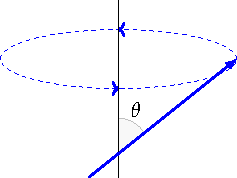
\includegraphics[]{Images/fig-spinprecess.pdf}

    \caption{When the initial spinor state $\chi(t = 0)$ is given by Eq. \eqref{eq-chithetat0} and evolves under a $z$-oriented magnetic field, the spin state can be visualized as precessing at fixed $\theta$ (the same $\theta$ as in the initial state). More technically, we could say that the spin state precesses at a fixed polar angle on the Bloch sphere; Note that the general spin state given in Eq. \eqref{eq-chigeneral} invites the visualization of a single spin-1/2 particle as a point on the unit sphere with polar coordinates $(\theta, \phi)$ (of course the global phase $\alpha$ is physically irrelevant).}
    \label{fig-spinprecess}
\end{figure}

However, there is a \emph{much} easier way to see why there is no time-dependence in the $S_z$ case, while there is a time-dependence in the $S_x$ case. The way to see this is that $[S_z, H] = 0$ ($S_z$ commutes with the Hamiltonian) so there is no time-dependence. Conversely, $S_x$ does not commute with the Hamiltonian, so we know that there is time dependence.

Let us discuss the simple case where:
\begin{equation}
    \chi(t = 0) = \frac{1}{\sqrt{2}}
    \m{1\\1}.
\end{equation}

Now, we want the probability of finding the spin to be in spin-up $P_\uparrow$ as a function of time. In this case, this will again be independent of time; a physical picture is that the spin precesses at a fixed angle, so the projection onto the $s_z$ axis does not change with time. A more concrete argument is that if we measure the probability of getting some outcome of an $S_z$ measurement, since $S_z$ commutes with $H$ then this probability should be independent of time. Let's see how this works out explicitly:
\begin{equation}
    \chi(t) = \frac{1}{\sqrt{2}}\m{1\\0}e^{i\omega t/2} + \frac{1}{\sqrt{2}}\m{0\\1}e^{-i\omega t/2}.
\end{equation}
By the Born rule we have::
\begin{equation}
    P_\uparrow = \abs{\braket{\uparrow}{\chi}}^2 = \frac{1}{2}
\end{equation}
which is time-independent. Let us now ask the probability of measuring $P_{+\xhat}$; how do we proceed? We start by finding the eigenstates of $S_x$:
\begin{equation}
    S_x \ket{\chi_{+\xhat}} = \lambda \ket{\chi_{+\xhat}} \cong \frac{1}{2}\sigma_x\chi_{+\xhat} = \lambda \chi_{+\xhat} \implies \chi_{+\xhat} = \frac{1}{\sqrt{2}}\m{1\\1}.
\end{equation}
We therefore can calculate:
\begin{equation}
    P_{+\xhat} = \abs{\frac{1}{\sqrt{2}}\m{1 & 1}\chi(t)}^2 = \abs{\frac{1}{\sqrt{2}}\m{1 & 1}\frac{1}{\sqrt{2}}\m{e^{i\omega t/2} \\ e^{-i\omega t/2}}}^2 = \abs{\frac{1}{2}\left(e^{i\omega t/2} + e^{-i\omega t/2}\right)}^2 = \frac{1}{2}\left(1 + \cos\omega t\right)
\end{equation}
Because the measurement is dichotomic, we can use completeness to find $P_{-\xhat}$:
\begin{equation}
    P_{-\xhat} = 1 - P_{+\xhat} = \frac{1}{2}\left(1 - \cos\omega t\right).
\end{equation}
\newpage
\section{Electromagnetic Fields}
\subsection{The Hamiltonian and Gaussian units}
We consider the Hamiltonian:
\begin{equation}\label{eq-Hem}
    H = \frac{1}{2m}\left(\v{p} - \frac{q}{c}\v{A}\right)^2 + qV
\end{equation}
We use Gaussian units, where $\frac{e^2}{4\pi \e_0} \to e^2$. The potential will (for the Coulomb interaction) will later be $qV = -\frac{Ze^2}{r}$ (the sign will be relevant later, to distinguish attractive (negative sign) and repulsive). For now take $q = -e$. Note for the magnetic moment we take:
\begin{equation}
    \mu = \frac{\abs{e}\hbar}{2mc}
\end{equation}
why Gaussian units? Because in SI units, the electric and magnetic fields have different units, but in Gaussian, they have the same units. Things will become unbelievably tedious to keep track of if we keep the $4\pi\e_0$s in. The Hydrogen atom Hamiltonian takes the form:
\begin{equation}
    H = \frac{1}{2m}\v{p}^2 - \frac{Ze^2}{r}.
\end{equation}
And to solve this problem, we take $\v{p} \to -i\hbar \nabla$ and use the standard techniques (covered in undergrad QM).

\subsection{Potentials and Gauge Invariance}
Let us make some comments about the Hamilonian in Eq. \eqref{eq-Hem}. We may be familiar with the Lorentz force law in classical E\&M:
\begin{equation}
    m\ddot{\v{r}} = \v{F} = q(\v{E} + \v{v} \times \v{B})
\end{equation}
where the dynamics are completely governed by the fields $\v{E}, \v{B}$. We can specify the fields by the scalar/vector potentials $V/\v{A}$:
\begin{equation}
    \v{B} = \nabla \times \v{A}, \quad \v{E} = -\nabla V - \frac{1}{c}\dpd{\v{A}}{t}.
\end{equation}
$V, \v{A}$ have features known as \emph{Gauge invariance}; a fundamental principle of nature. Consider the gauge transformation:
\begin{equation}
    V' = V - \frac{1}{c}\dpd{f(\v{r}, t)}{t}, \quad \v{A}' = \v{A} + \nabla f(\v{r}, t).
\end{equation}
When we do computations for electric and magnetic fields, we find that $V'/\v{A}'$ specify the same physical fields:
\begin{equation}
    \v{E}' = -\nabla V' - \frac{1}{c}\dpd{\v{A}'}{t} = \v{E} + \left(\dpd{}{t}\nabla  - \nabla \dpd{}{t}\right)f(\v{r}, t) = \v{E}
\end{equation}
and analogously:
\begin{equation}
    \v{B}' = \v{B}.
\end{equation}
In classical physics, this is a triviality; a gauge transformation does nothing to the physics. What about quantum mechanics? In quantum mechanics we solve the SE:
\begin{equation}
    H\psi = E\psi
\end{equation} 
with the Hamiltonian Eq. \eqref{eq-Hem}. Now it begins to seem like we have a different equation; is this indeed the case? 

In classical physics, we tend to fix gauges based on convenience. When we study electrostatics, we choose the Coloumb gauge:
\begin{equation}
    \nabla \cdot \v{A} = 0
\end{equation}
When we study radiation, we choose the Lorentz gauge (convenient as it is Lorentz covariant):
\begin{equation}
    \nabla \cdot \v{A} + \frac{1}{c}\dpd{V}{t} = 0.
\end{equation} 
We mention this as we want a quantum-classical correspondence; we want to be able to compare the quantum and classical calculation at the end.

\subsection{QM Resolution of the Problem}
Let us precisely study what happens when we change the Gauge.
\begin{equation}
    \left(\v{p}' - \frac{q}{c}\v{A}'\right)\psi'
\end{equation}
where:
\begin{equation}
    \psi' = e^{i\frac{q}{\hbar c}f}\psi
\end{equation}
If there is no degeneracy, we have no problem as changing the Gauge only introduces a physically meaningless phase; however the problem appears when we have degeneracy (e.g. in the Landau levels HW problem; we have an infinite degeneracy). Let us study this further:
\begin{equation}
    -i\hbar \nabla \psi' - \frac{q}{c}A'\psi' = -i\hbar \nabla\psi e^{i\frac{q}{\hbar c}t} + \frac{q}{c}(\nabla f)e^{i\frac{q}{\hbar c}f}\psi - \frac{q}{c}\v{A}\psi e^{i\frac{q}{\hbar c}f} - \frac{q}{c}(\nabla f)e^{i \frac{q}{\hbar c}f}\psi
\end{equation}
The second and fourth terms cancel, so we have:
\begin{equation}
    \left(\v{p}' - \frac{q}{c}\v{A}'\right)\psi' = \left[\left(\v{p} - \frac{q}{c}\v{A}\right)\psi\right]e^{i\frac{q}{\hbar c}f}
\end{equation}
We therefore obtain the following: when we do the SE, the phase appears on the LHS and RHS, and cancels. So though the Hamiltonian may be different, the eigenfunctions are the same. So we say that the covariant derivative $\left(\v{p} - \frac{q}{c}\v{A}\right)$ is gauge invariant. If we break gauge invariance, then we break fundamental principles.

\subsection{}
We work with the Hamiltonian:
\begin{equation}
    H = \frac{1}{2m}\left(\v{p} - \frac{q}{c}\v{A}\right)^2
\end{equation}
where we have neglected the trivial $V$ term (if we have a time-independent gauge transformation, the $V$ remains unchanged). Let us write this in tensorial notation:
\begin{equation}
    H = \frac{1}{2m}\left(\v{p}_i - \frac{q}{c}\v{A}_i\right)\left(\v{p}_i - \frac{q}{c}\v{A}_i\right)
\end{equation}
We can represent this as follows:
\begin{equation}
    H = \frac{1}{2m}\left(\v{p}^2 + \left(\frac{q}{c}\v{A}\right)^2 - \frac{q}{c}\left(\v{A} \cdot \v{p} + \v{p}\cdot\v{A}\right)\right)
\end{equation}
Now we want to calculate $[p_i, A_j]$. Let us build up to this. We know already that:
\begin{equation}
    [p_x, x] = -i\hbar
\end{equation}
We can derive:
\begin{equation}
    [p_i, f(\v{r})] = -i\hbar \nabla_i f(\v{r})
\end{equation}
where the RHS is determined by explicitly writing out the commutator and acting it on a test function (alternatively: taylor expand the $f$ and use induction). Directly applying this we have:
\begin{equation}
    [p_i, A_j(\v{r})] = -i\hbar \nabla_i A_j(\v{r}).
\end{equation}

Now, pay attention to how we fix the Gauge:
\begin{equation}
    \delta_{ij}[p_i, A_j(\v{r})] = -i\hbar \nabla_i A_j(\v{r})\delta_{ij}
\end{equation}
so then:
\begin{equation}
    [p_i, A_j] = -i\hbar \nabla \cdot \v{A} = 0.
\end{equation}
so we work in the Coloumb gauge, where $p_i, A_j$ commute (note this is NOT true in any other gauge). So our Hamiltonian in this gauge becomes:
\begin{equation}
    H =  H = \frac{1}{2m}\left(\v{p}^2 + \left(\frac{q}{c}\v{A}\right)^2 - \frac{2q}{c}\v{A} \cdot \v{p}\right).
\end{equation}
We have the vector potential:
\begin{equation}
    \v{A} = -\frac{1}{2}\v{r} \times \v{B}
\end{equation}
and we work in a cylindrical system, with $A_z = 0, A_r = 0, A_\phi = \frac{1}{2}rB_z$. The magnetic field is calculated to be:
\begin{equation}
    \v{B} = \nabla \times \v{A} = \frac{1}{r}\left[\dpd{}{r}(rA_\phi) - \dpd{}{\phi}A_r\right]\zhat = \frac{1}{r}\dpd{r^2B_z/2}{r} = B_z
\end{equation}
(it can be checked that the radial/angular parts of the magnetic field are zero). We compute the $\v{A} \cdot \v{p}$ term:
\begin{equation}
    \v{A} \cdot \v{p} = -\frac{1}{2}\left(\v{r} \times \v{B}\right) \cdot \v{p} = \frac{1}{2}\v{B} \cdot (\v{r} \times \v{p}) = \frac{1}{2}\v{B} \cdot \v{L}.
\end{equation}
So the term in the Hamiltonian is:
\begin{equation}
    -\frac{2q}{2mc}\v{A} \cdot \v{p} = -\frac{q}{mc}\frac{1}{2}\v{B} \cdot \v{L} = -\gv{\mu} \cdot \v{B}
\end{equation}
where we have taken:
\begin{equation}
    \gv{\mu} = \mu \v{L} = \frac{q}{2mc}\v{L}
\end{equation}
So we find the gyromagnetic ratio:
\begin{equation}
    \mu = \frac{q\hbar}{2mc}.
\end{equation}
where we take $\hbar$ to be included in the $\mu$ so we can work with angular momentum dimensionlessly.
\newpage
\section{Gauge Invariance Part II, Angular Momentum Addition}
\subsection{Gauge Invariance, Symmetry, Conservation Laws}
In addition to the gauge invariance we are familiar from classical electromagnetism, in QM we get an extra phase factor:
\begin{equation}
    \psi' = e^{i\frac{q}{\hbar c}f}\psi.
\end{equation}
If the wavefunction describes a single state (no degeneracy), then we can ignore this global phase. But normally we do have degeneracy (and often infinite degeneracy), and here this phase factor will be significant. See HW1Q9 for a concrete example of this.

Why do we go on about gauge invariance? Because gauge invariance is connected to some symmetry (which leads to a conserved quantity via Noether's theorem). In this case, the conserved quantity is charge. We are familiar with the examples of momentum being conserved due to translation invariance, angular momentum being conserved due to rotational invariance, and energy being conserved due to time invariance. 

\subsection{Analyzing the Coulomb Hamiltonian}
We recall the Hamiltonian, with the choice of Coulomb gauge $\nabla \cdot \v{A} = 0$.
\begin{equation}
    H = \left(\v{p} - \frac{q}{c}\v{A}\right)^2\frac{1}{2m} = \frac{1}{2m}\left(\v{p}^2 + \frac{q^2}{c^2}\v{A}^2 - \frac{2q}{c}\v{A}\cdot \v{p}\right)
\end{equation}
If we have $\v{A} = \frac{1}{2}\v{r} \times \v{B}$, $\v{A}$ gives us the correct magnetic field. We recall that the $\v{A} \cdot \v{p}$ term precisely describes the interaction of the magnetic moment with the magnetic field:
\begin{equation}
- \frac{2q}{c}\v{A}\cdot \v{p} \to \frac{q}{2mc} B_zL_z.
\end{equation}
We have not introduced spin here, as this would be more complicated (we would be working with the Dirac equation, and work with an extra $+2S_z$ piece). If we represent $\v{A}^2$ in terms of what we did last class, we can write the entire Hamiltonian as:
\begin{equation}
    H = \frac{p_z^2}{2m} + \left(\frac{p_x^2 + p_y^2}{2m} + \frac{q^2B^2}{8mc^2}\left(x^2 + y^2\right)\right) - \frac{q}{2mc}B_zL_z
\end{equation}
we note the structure of the above expression; we have three terms:
\begin{equation}
    H_z = \frac{p_z^2}{2m}, \quad H_\perp = \left(\frac{p_x^2 + p_y^2}{2m} + \frac{q^2B^2}{8mc^2}\left(x^2 + y^2\right)\right), \quad H_{\parallel} =  - \frac{q}{2mc}B_zL_z
\end{equation}
We don't have to solve the Hamiltonian, which is very complicated. We instead sit down and look at it. In particular, we want to know what operators commute with the Hamiltonian. First, we see:
\begin{equation}
    [H, p_z] = 0
\end{equation}
as there are no terms with $z$ in the Hamiltonian. So, the $z$-momentum is a conserved quantity, and the eigenstates in $z$ are plane waves. Next, we have that:
\begin{equation}
    [H, L_z] = 0.
\end{equation}
How do we see this? The Hamiltonian is \emph{radially symmetric}, i.e. although $L_z$ has a nontrivial commutator with $x, y$, it commutes with $x^2 + y^2 = r^2$. Next, we ask whether we can measure $p_z$ and $L_z$ simultaneously; of course we can:
\begin{equation}
    [p_z, L_z] = 0.
\end{equation}
The next question we ask; we have $H_\perp$ which is the Hamiltonian in the plane. We already have argued that:
\begin{equation}
    [L_z, H_\perp] = 0.
\end{equation}
We now have an equation that we can immediately solve. Our state is classified by three different numbers; first:
\begin{equation}
    p_z\psi_k = \hbar k \psi_k.
\end{equation}
where:
\begin{equation}
    \psi_k =  e^{i\frac{p_z z}{\hbar}} = e^{i\frac{\hbar k z}{\hbar}}.
\end{equation}
We also have:
\begin{equation}
    L_z\ket{l} = \hbar l \ket{l}
\end{equation}
(and we already know what the eigenstates look like). We also have the third term:
\begin{equation}
    H_\perp \psi_n = E_n \psi_n
\end{equation}
but we can see by inspection that $H_\perp$ is nothing but a two-dimensional quantum harmonic oscillator, so:
\begin{equation}
    E_n = \hbar \omega (n + 1), \quad n = (n_x + \frac{1}{2}) + (n_y + \frac{1}{2}).
\end{equation}
where $\omega$ is as usual defined as:
\begin{equation}
    \omega^2 = \frac{q^2B^2}{4mc^2}\frac{1}{m} = \left(\frac{qB}{2mc}\right)^2.
\end{equation}
$\omega$ is nothing more than the Larmour frequency which we know from classical electromagnetism. What is important is to look at the expression for $H_\parallel$; it is precisely the Larmour frequency which appears. So, writing down the final expression for the energy, we have:
\begin{equation}
    E_{klm} = \hbar \omega(n + l + 1) + \frac{\hbar^2 k^2}{2m}
\end{equation}
Where the $n + 1$ comes from the $H_\perp$ term, the $l$ comes from the $H_\parallel$ term, and the $k$ comes from the $H_z$ term. Once we look at this expression (taking $k = 0$ for expression), we see a \emph{huge} degeneracy, as $l$ goes over integer values, and $n$ goes from $0$ to $\infty$ (note we have the constraint that $(n + l) \geq 0$ as $H$ is positively defined). We define:
\begin{equation}
    N \coloneqq n + l + 1
\end{equation}
and so we get:
\begin{equation}
    E_{0N} = \hbar \omega N.
\end{equation}

In HW1Q9, we go through the same calculation in a different gauge. We will see that there are infinitely many degenerate states, in a different basis when solved in a different gauge (but this is not a problem, as of course we can just express these different eigenfunctions in a different basis).

\subsection{Addition of Angular Momentum - Motivation}
In nature, we have many interactions that are not taken into account in the SE. For example, we have the magnetic moment-magnetic moment interaction:
\begin{equation}
    \Delta V = \frac{-\gv{\mu}_1 - \gv{\mu}_2}{r^3} \sim \v{S}_1 \cdot \v{S}_2
\end{equation}
this is the spin-spin interaction, also known as exchange forces in condensed matter physics. We also can have spin-orbit interactions of:
\begin{equation}
    \Delta V \sim \v{S} \cdot \v{L}
\end{equation}
There is no way to understand the periodic table, spectra, or transitions without understanding these interactions. What is the starting point when we ignore this interaction? When we discuss the hydrogen atom, we solve:
\begin{equation}
    H = \frac{\v{p}^2}{2m} - \frac{e^2}{r}.
\end{equation}
Here we see no sign of the spin-orbit interactions. We classify all states by three quantum numbers, $n$ (principle) $l$ (orbital) $m$ (projection of orbital). If we introduce spin (but not include it in the Hamiltonian), we can introduce a $s = 1/2, s_z = \pm 1/2$ into our state:
\begin{equation}
    \ket{n, l, m, s = \frac{1}{2}, s_z = \pm \frac{1}{2}}.
\end{equation}
Now we ask; is this a good or bad classification of states? Let us for take our spin orbit interaction:
\begin{equation}
    \Delta V = \v{S} \cdot \v{L}.
\end{equation}
Does spin commute or not commute with the spin orbit interaction? It of course does not as $S_i$ will not commute with the other components. So:
\begin{equation}
    [S_i, \v{S} \cdot \v{L}] \neq 0, [L_i, \v{S} \cdot \v{L}] \neq 0.
\end{equation}
This is why we need a better classification of states. We consider:
\begin{equation}
    \Delta V = \v{S}^{(1)} \cdot \v{S}^{(2)}
\end{equation}
we then have:
\begin{equation}
    [S^{(1)}_i, \Delta V] = [S_i^{(1)}, S_j^{(1)}S_j^{(2)}] = [S_i^{(1)}, S_j^{(1)}]S_j^{(2)} = i\e_{ijk}S_k^{(1)}S_j^{(2)}.
\end{equation}
We now do the computations for $S_2$:
\begin{equation}
    [S_i^{(2)}, \Delta V] = [S_i^{(2)}, S_j^{(1)}S_j^{(2)}] = S_j^{(1)}[S_i^{(2)}, S_j^{(2)}] = i\e_{ijk}S_j^{(1)}S_k^{(2)}.
\end{equation}
We now consider the following. If we introduce:
\begin{equation}
    \v{S}^{tot} = \v{S}^{(1)} + \v{S}^{(2)}
\end{equation}
then we see that $\v{S}^{tot}$ commutes with the interaction:
\begin{equation}
    [S_i^{(1)} + S_i^{(2)}, \Delta V] = i\e_{ijk}S_k^{(1)}S_j^{(2)} + i\e_{ijk}S_j^{(1)}S_k^{(2)}
\end{equation}
We now do a trick, where we exchange $j$ and $k$; it does not matter as we sum over all of them:
\begin{equation}
    [S_i^{(1)} + S_i^{(2)}, \Delta V] = i\e_{ijk}S_k^{(1)}S_j^{(2)} + i\e_{ikj}S_k^{(1)}S_j^{(2)}
\end{equation}
then we introduce a minus sign by swapping $j$ and $k$ in the Levi-Civita symbol:
\begin{equation}
    [S_i^{(1)} + S_i^{(2)}, \Delta V] = i\e_{ijk}S_k^{(1)}S_j^{(2)} - i\e_{ijk}S_k^{(1)}S_j^{(2)} = 0.
\end{equation}
So, we can deduce a better classification of our states:
\begin{equation}
    \ket{n, l, s = \frac{1}{2}, J, J_z}
\end{equation}
where:
\begin{equation}
    \v{J} = \v{L} + \v{S}.
\end{equation}
We will discuss this basis further next class.
\newpage
\section{Addition of Angular Momentum, Continued}
\subsection{Review of Last Class}
We represent all magnetic-moment coupling interactions as:
\begin{equation}
    \Delta V = \v{S}^{(1)} \cdot \v{S}^{(2)}
\end{equation}
Where the coupling constant has been set to unity. We then found:
\begin{equation}
    [S_i^{(1)}, \Delta V] \neq 0, [S_i^{(2)}, \Delta V] \neq 0.
\end{equation}
But did find that the total angular momentum $S_i^{tot} = S_i^{(1)} + S_i^{(2)}$ did commute:
\begin{equation}
    [S_i^{tot}, \Delta V] = 0.
\end{equation}
From this, we concluded that the classification of hydrogen atom states based on the quantum numbers $\ket{n, l, m, s=1/2, s_z}$ was a bad classification; instead, a better classification is $\ket{n, l, s= 1/2, J, J_z}$, where:
\begin{equation}
    \v{J} = \v{L} + \v{S}.
\end{equation}
This is a good classification sense in the operators corresponding to each of the quantum numbers commute with each other and the Hamiltonian. Note that the $J_i$s also follow the angular momentum algebra:
\begin{equation}
    [J_i, J_j] = i\e_{ijk}J_k.
\end{equation}
This can be verified by their definition:
\begin{equation}
    [J_i, J_j] = [L_i + S_i, L_j + S_j] = [L_i, L_j] + [S_i, S_j] = i\e_{ijk}(L_k + S_k) = i\e_{ijk}J_k.
\end{equation}
Hence our general results proven previously for arbitrary angular momentum operators still hold, i.e.:
\begin{equation}
    [\v{J}^2, J_i] = 0
\end{equation}
and all of the commutation relations with $J_\pm, J_z$ etc.

\subsection{Adding Two Spin-1/2 Particles}
In practice, when adding up angular momenta we can just refer to tables (or computer programs) which tabulate Clebsch-Gordon coefficients, which tell us how states in the $\ket{s^{(1)}, s^{(2)}, s, s_z}$ basis (where $s$ is the joint spin) can  expanded in state in the $\ket{s^{(1)}, s_z^{(1)}, s^{(2)}, s_z^{(2)}}$ basis (and vise versa). We discuss the simplest case here, with $s^{(1)} = 1/2, s^{(2)} = 1/2$. Also from now on we suppress the $s^{(1)}, s^{(2)}$ as these always remain unchanged (always $1/2$). Also note the notation:
\begin{equation}
    \ket{\uparrow} \otimes \ket{\uparrow} = \ket{\uparrow\uparrow} \cong \m{1\\0} \otimes \m{1\\0} = \m{1\\0\\0\\0}.
\end{equation}
Can we immediately say how $\ket{\uparrow\uparrow}$ will be expressed in the $\ket{s, s_z}$ basis? Yes. 
\begin{equation}
    \ket{\uparrow \uparrow} \mapsto \ket{s = 1, s_z = + 1}.
\end{equation}
Why is $s = 2$ not possible here? This is because that would (of course) violate angular momentum conservation. The $\ket{\downarrow\downarrow}$ works out in the same way:
\begin{equation}
    \ket{\downarrow\downarrow} \mapsto \ket{s = 1, s_1 = -1}.
\end{equation}
We now consider applying the raising and lowering operators to these states. In particular, we apply them in two different forms. First, applying this in the joint basis, we know that:
\begin{equation}
    S_-\ket{\uparrow\uparrow} = \sqrt{2}\ket{s = 1, s_z = 0}
\end{equation}
The constant was determined by using the coefficients of the raising/lowering operators derived in the second class. Applying $S_-$ in the form $S_- = S_-^{(1)} + S_-^{(2)}$ we have:
\begin{equation}
    S_-\ket{\uparrow\uparrow} = (S_-^{(1)} + S_-^{(2)})\ket{\uparrow} = \ket{\downarrow\uparrow} + \ket{\uparrow\downarrow}.
\end{equation}
Where again the coefficients can be obtained by the general raising/lowering coefficient formula. Comparing the two expressions, we find:
\begin{equation}
    \ket{s = 1, s_z = 0} = \frac{\ket{\uparrow\downarrow} + \ket{\downarrow\uparrow}}{\sqrt{2}}.
\end{equation}

Now, let's back up a bit. In the $\ket{s^{(1)}, s_z^{(1)}, s^{(2)}, s_z^{(2)}}$ basis, we have three basis states; $2 \times 2 = 4$ as each spin has two basis states (explicitly, a basis is $\ket{\uparrow\uparrow}, \ket{\uparrow\downarrow}, \ket{\downarrow\uparrow}, \ket{\downarrow\downarrow}$). However, in our construction of the $\ket{s, s_z}$ basis, we have only constructed three states. What is the fourth?

We need to find the last state. This last state will have $s = 0$ (this is the only possibility left). How do we construct it? We can find it via the following observation; the state $\ket{s = 0, s_z = 0}$ must be \emph{orthogonal to all of the other three states found so far, as it has a different quantum number $s$}. Note that it is immediate to see that:
\begin{equation}
    \braket{\uparrow\uparrow}{s=0, s_z = 0} = \braket{\downarrow\downarrow}{s=0, s_z=0} = 0
\end{equation}
as $\ket{s = 0, s_z = 0}$ must be constructed out of parts that have spin-$z$ projection zero, i.e. it must be constructed out of states $\ket{\uparrow\downarrow}$ and $\ket{\downarrow\uparrow}$ (which are orthogonal to $\ket{\uparrow\uparrow}$ and $\ket{\downarrow\downarrow}$). So, we find the coefficients $a, b$ in:
\begin{equation}
    \ket{s=0, s_z = 0} = a\ket{\uparrow\downarrow} + b\ket{\downarrow\uparrow}
\end{equation}
And we require this to be orthogonal to $\ket{s=1, s_z = 0}$, so:
\begin{equation}
    \frac{1}{\sqrt{2}}\left(\bra{\uparrow\downarrow} + \bra{\downarrow\uparrow}\right)\left( a\ket{\uparrow\downarrow} + b\ket{\downarrow\uparrow}\right)
\end{equation}
and after doing the computation (and normalization of the coefficients), I find that $a = 1/\sqrt{2}, b = -1/\sqrt{2}$ and so:
\begin{equation}
    \ket{s=0, s_z = 0} = \frac{\ket{\uparrow\downarrow} - \ket{\downarrow\uparrow}}{\sqrt{2}}.
\end{equation}
So we have succeeded in constructing the four states in the $\ket{s, s_z}$ basis. Our classification is complete.

\subsection{Checking Joint Set Properties}
Let us check that indeed the $\ket{s=0, s_z = 0}$ state we constructed has spin zero. We consider the operator:
\begin{equation}
    \v{S}^2 = \left(\v{S}^{(1)} + \v{S}^{(2)}\right)^2 = (\v{S}^{(1)})^2 + (\v{S}^{(2)})^2 + 2\v{S}^{(1)} \cdot \v{S}^{(2)} =  (\v{S}^{(1)})^2 + (\v{S}^{(2)})^2 + 2S_z^{(1)}S_z^{(2)} + S_+^{(1)}S_-^{(2)} + S_-^{(1)}S_+^{(2)}
\end{equation}
Since the joint spin satisfies the angular momentum algebra, we already expect that:
\begin{equation}
    \v{S}^2\ket{s = 1, s_z = 0} = 1(1+1)\ket{s=1, s_z = 0} = 2\ket{s=1, s_z = 0}
\end{equation}
\begin{equation}
    \v{S}^2\ket{s=0, s_z=0} = 0.
\end{equation}
Let's apply $\v{S}^2$ to $\ket{\uparrow\downarrow}$. We go term by term:
\begin{equation}
    (\v{S}^{(1)})^2\ket{\uparrow\downarrow} = \frac{3}{4}\ket{\uparrow\downarrow}
\end{equation}
\begin{equation}
    (\v{S}^{(2)})^2\ket{\uparrow\downarrow} = \frac{3}{4}\ket{\uparrow\downarrow}
\end{equation}
\begin{equation}
   2S_z^{(1)}S_z^{(2)}\ket{\uparrow\downarrow} = 2\frac{1}{2}\cdot \frac{-1}{2}\ket{\uparrow\downarrow} = -\frac{1}{2}\ket{\uparrow\downarrow}
\end{equation}
\begin{equation}
    S_+^{(1)}S_-^{(2)}\ket{\uparrow\downarrow} = 0.
\end{equation}
\begin{equation}
    S_-^{(1)}S_+^{(2)}\ket{\uparrow\downarrow} = \ket{\downarrow\uparrow}
\end{equation}
so in total:
\begin{equation}
    \v{S}^2\ket{\uparrow\downarrow} = \ket{\uparrow\downarrow} + \ket{\downarrow\uparrow}.
\end{equation}
And analogously, we find:
\begin{equation}
    \v{S}^2\ket{\uparrow\downarrow} = \ket{\downarrow\uparrow} + \ket{\uparrow\downarrow}.
\end{equation}
so then:
\begin{equation}
    \v{S}^2\left(\ket{\downarrow\uparrow} + \ket{\uparrow\downarrow}\right) = 2\left(\ket{\downarrow\uparrow} + \ket{\uparrow\downarrow}\right)
\end{equation}
which is exactly what we predicted.

\subsection{Adding a Spin-1 and Spin-1/2 Particle}
We take $l = 1, s = \frac{1}{2}$, and take $\v{J} = \v{L} + \v{S}$. The number of states is $(2l + 1)(2s + 1) = 3\cdot 2 = 6$. We immediately have:
\begin{equation}
    \ket{l_z = 1, s_z = \frac{1}{2}} = \ket{J = \frac{3}{2}, J_z = \frac{3}{2}}.
\end{equation}
There are four states total with $J = \frac{3}{2}$ ($J_z = \frac{3}{2}, \frac{1}{2}, \frac{-1}{2}, \frac{-3}{2}$) and two more states with $J = \frac{1}{2}$ ($J_z = \frac{1}{2}, \frac{-1}{2}$). For the rest of the states with $J = \frac{3}{2}$, we can apply $J_-$ to the maximal projection state with $J_z = \frac{3}{2}$ above.
\begin{equation}
    J_-\ket{l_z = 1, s_z = \frac{1}{2}} \sim \ket{J = \frac{3}{2}, J_z = \frac{1}{2}}
\end{equation}
Explicitly:
\begin{equation}
    (L_- + S_-)\ket{l_z = 1, s_z = \frac{1}{2}} = \sqrt{2}\ket{l_z = 0, s_z = \frac{1}{2}} + 1\ket{l_z = 1, s_z = -\frac{1}{2}}
\end{equation}
So normalizing:
\begin{equation}
    \ket{J = \frac{3}{2}, J_z = \frac{1}{2}} = \frac{\sqrt{2}\ket{l_z = 0, s_z = \frac{1}{2}} + 1\ket{l_z = 1, s_z = -\frac{1}{2}}}{\sqrt{3}}
\end{equation}
and we can go on. Next time, we briefly discuss the general case, and how to construct the wavefunctions of the hydrogen atom properly.

\newpage
\section{Addition of Angular Momentum (Concluded), Time-Independent Perturbation Theory}

\subsection{General Theory of Addition of Angular Momentum}
Last time, we covered a few simple examples (spin-1/2 + spin-1/2 and spin-1/2 + spin-1) of angular momentum addition. Now, we proceed with a brief discussion of the general case, where we add a spin-$s_1$ particle to a spin-$s_2$ particle. We then have the relation:
\begin{equation}
    \ket{s m} = \sum_{m = m_1 + m_2} C_{m m_1 m_2}^{s s_1 s_2}\ket{s_1m_1}\ket{s_2m_2}
\end{equation}
where $s$ is the joint spin, $m = m_1 + m_2$ is the joint spin-$z$ component, and the $C_{m m_1 m_2}^{s s_1 s_2}$s are the Clebsch-Gordon coefficients (a table of which can be found in literally any quantum mechanics textbook). 

We return to the question of degeneracy. The number of states in the $\ket{s_1m_2}\ket{s_2m_2}$ basis is given by $(2s_1 + 1)(2s_2 + 1)$. We can then count the degeneracy in the $\ket{sm}$ basis as:
\begin{equation}
    (2s_1 + 1)(2s_2 + 1) = \sum_{s_{min} = \abs{s_1 - s_2}}^{s_{max} = \abs{s_1 + s_2}}(2s+1)
\end{equation}
Let's look at this formula for a couple examples. For $s_1 = s_2 = \frac{1}{2}$ we have:
\begin{equation}
    2 \cdot 2 = 1 + 3
\end{equation}
w here the first term corresponds to $s = 0$ and the second term corresponds to $s = 1$. For $s_1 = \frac{1}{2}$ and $s_2 = 1$ we have:
\begin{equation}
    3 \cdot 2 = 2 + 4
\end{equation}
where the first term corresponds to $s = \frac{1}{2}$ and the second term corresponds to $s = \frac{3}{2}$. We also discussed why we cannot exceed $s = \abs{s_1 + s_2}$; it comes down to rotational symmetry and angular momentum conservation.

In general, do not waste time computing CGCs (although the procedure to do so was illustrated last class, and you have one example in the homework); people have tabulated all of these coefficients already, and you can look them up.

\subsection{Classification of Hydrogen Atom States}
Normally, when we do computations with the Hydrogen atom, we have $\ket{n, l, m, s=1/2, s_z}$. But this is not a good basis (discussed last class) so we consider instead the basis $\ket{n, l, s=1/2, J, J_z}$. We use spectroscopic notation $n\prescript{2s+1}{}{L}_J$. For the hydrogen atom we always have $s = 1/2$ so we can omit this and write $nL_J$. We can write the energy levels as per the diagram below:

\begin{table}[htbp]
    \centering\begin{tabular}{|c|c|c|c|}
        \hline Old Classification & Degeneracy Counting (Old) & New classification & Degeneracy Counting (New)
        \\ \hline 3s3p3d & 2 + 6 + 10 = 18 & $3s_{1/2}$ (2) $3p_{1/2}$ (2) $3p_{3/2}$ (4) $3d_{3/2}$ (4) $3d_{5/2}$ (6) & 2 + 2 + 4 + 4 + 6 = 18
        \\ \hline 2s2p & 2 + 6 = 8 & $2s_{1/2}$ (2) $2p_{1/2}$ (2) $2p_{3/2}$ (4) & 2 + 2 + 4 = 8
        \\ \hline 1s & 2 = 2 & $1s_{1/2}$ (2) & 2 = 2
        \\ \hline
    \end{tabular}
    \caption{Spectroscopic classificatio of states of the hydrogen atom. On the left is the old classification, with $s$ having two states (corresponding to $l = 0$ and so $J = 1/2$ (2)), $p$ having six states (corresponding to $l = 1$ and so $J = 3/2$ (4) and $J = 1/2$ (2)), and $d$ having 10 states (corresponding to $l = 2$ and so $J = 5/2$ (6), $J = 3/2$ (4) and $J = 1/2$ (2)). On the right is the new classification, which quantifies the states according to our better new set of quantum numbers. The degeneracy in the two cases is the same.}
    \label{table-Hclassification}
\end{table}

A fun little aside; D-wave (the quantum computing company in Burnaby) got its name from the d-waves inside high-$T_c$ superconductors, which they were working on when the company was started.

5 second question: Why is there no $d = 1/2$? Because the minimum is $s = \abs{s_1 - s_2} = \abs{2 - \frac{1}{2}} = \frac{3}{2}$. 

In conclusion, we see that the true classification is based on the joint angular momentum. Let us see how we construct the wavefunctions corresponding to different states:
\begin{equation}
    1s_{1/2} \cong R_{10}Y_0^0\m{1\\0}.
\end{equation}
How do we construct the other states? We can use Clebsch-Gordon coefficients:
\begin{equation}
    2p_{1/2}(J_z = \frac{1}{2}) = \sqrt{\frac{2}{3}}\ket{1\frac{-1}{2}} - \sqrt{\frac{1}{3}}\ket{0\frac{1}{2}} \cong \sqrt{\frac{2}{3}}R_{21}Y_1^1\m{0\\1} - \sqrt{\frac{1}{3}}R_{21}Y_1^0\m{1\\0}.
\end{equation}
The probability of finding spin-up is $\frac{1}{3}$. The probability of finding spin-up in some region can be found by integrating $R_{21}Y_1^0$ over a given spatial region. The probability of finding total angular momentum can also be calculated by reversing the Clebsch-Gordon table (it can be read both ways, depending on whether one goes by column or by row).

\subsection{Non-Degenerate Time-Independent Perturbation Theory}
Why do we want PT? Many systems are not analytically solvable\footnote{Indeed, the solvable problems are the free particle, the infinite box, the oscillator, and the hydrogen atom.}, but in many cases we have some kind of small parameter, for which we can treat as a perturbation and get an approximate result. Our starting point is the Hamiltonian:
\begin{equation}
    H = H^{(0)} + \lambda H^{(1)}
\end{equation}
where $H^{(0)}$ is an analytically solvable Hamiltonian, and $\lambda$ is a ``small'' parameter (we will comment on what this means later). We have the eigenfunctions/eigenenergies of $H^{(0)}$:
\begin{equation}
    H^{(0)}\psi^{(0)}_n = E_n^{(0)}\psi_n^{(0)}
\end{equation}
We expand the eigenfunctions and eigenenergies of $H$ in $\lambda$:
\begin{equation}
    \psi_n = \psi_n^{(0)} + \lambda \psi_n^{(1)} + \ldots, \quad E_n = E_n^{(0)} + \lambda E_n^{(1)} + \ldots
\end{equation}
The eigenvalue equation then reads:
\begin{equation}\label{eq-pertexpansion}
    (H^{(0)} + \lambda H^{(1)})(\psi_n^{(0)} + \lambda \psi_n^{(1)} + \ldots) = (E_n^{(0)} + \lambda E_n^{(1)} + \ldots)(\psi_n^{(0)} + \lambda \psi_n^{(1)} + \ldots).
\end{equation}
We can then collect the terms in orders of $\lambda$. The $\lambda^0 = 1$ terms read:
\begin{equation}
    H^{(0)}\psi^{(0)}_n = E_n^{(0)}\psi_n^{(0)}
\end{equation}
and of course these are just the eigenvalues/eigenfunctions of the exactly solvable Hamiltonian $H^{(0)}$. If we collect the terms in order $\lambda^1$, we find:
\begin{equation}
    E_n^{(1)} = \bra{\psi_n^{(0)}}H^{(1)}\ket{\psi_n^{(0)}}
\end{equation}
and if we collect the terms in order $\lambda^2$, we find:
\begin{equation}
    E_n^{(2)} = \sum_{m \neq n}\frac{\abs{\bra{\psi_m^{(0)}}H^{(1)}\ket{\psi_n^{(0)}}}}{E_m^{(0)} - E_n^{0}}.
\end{equation}
However we notice that when we have degeneracy, the second order energy corrections explode as $E_m^{(0)} = E_n^{(0)}$ for some $m \neq n$. So, our standard procedure only works for non-degenerate systems. However many systems of physical interest (such as the hydrogen atom) exhibit a large amount of degeneracy, so let's look at how to treat this problem.

\subsection{Degenerate Time-Independent Perturbation Theory}
If we have a degeneracy, then:
\begin{equation}
    H^{(0)}\psi_{a, b}^{(0)} = E^{(0)}\psi_{a, b}^{(0)}
\end{equation}
for some $a, b$. We can then immediately convince ourselves that:
\begin{equation}
    E_a^{(1)} = \bra{\psi_a^{(0)}}H^{(1)}\ket{\psi_a^{(0)}}, \quad E_b^{(1)} = \bra{\psi_b^{(0)}}H^{(1)}\ket{\psi_b^{(0)}}
\end{equation}
is wrong. Why? Because if we can use $a, b$, then we can use an arbitrary superposition:
\begin{equation}\label{eq-degenlinearcomb}
    \tilde{\psi}^{(0)} = \alpha\psi_a^{(0)} + \beta\psi_b^{(0)}
\end{equation}
but then the naive first-order correction could give any answer we want depending on what linear combination we take; of course this is wrong (things should be unique in physics). So let us repair this. We consider the case where the ground state is degenerate (but this procedure can be easily generalized). We go back to our expansion in Eq. \eqref{eq-pertexpansion} and replace $\psi_n^{(0)}$ with the linear combination \eqref{eq-degenlinearcomb}. We introduce matrix elements:
\begin{equation}
    \begin{split}
        T_{aa} &= \bra{\psi_0^a}H^{(1)}\ket{\psi_0^a}
        \\T_{ab} &= \bra{\psi_0^a}H^{(1)}\ket{\psi_0^b}
        \\T_{ba} &= \bra{\psi_0^b}H^{(1)}\ket{\psi_0^a}
        \\T_{bb} &= \bra{\psi_0^b}H^{(1)}\ket{\psi_0^b}
    \end{split}
\end{equation}
Having introduced this, we can proceed precisely the same way that we did in the non-degenerate case. If we do so, the equations we obtain are:
\begin{equation}
    \begin{split}
        &\alpha T_{aa} + \beta T_{ab} - \alpha E^{(1)} = 0
        \\ &\beta(T_{bb} - E^{(1)}) + \alpha T_{ba} = 0.
    \end{split}
\end{equation}
The claim now is that these equations cannot be satisfied for arbtirary $\alpha, \beta$; in particular, we require that:
\begin{equation}
    \det\m{T_{aa} - E^{(1)} & T_{ab} \\ T_{ba} & T_{bb} - E^{(1)}} = 0.
\end{equation}
i.e. $E^{(1)}$ is a eigenvalue of the $T$-matrix corresponding to eigenvector $\m{\alpha\\\beta}$. After going through the linear algebra, we find:
\begin{equation}
    E^{(1)}_\pm = \frac{1}{2}\left(T_{aa} + T_{bb}\right) \pm \frac{1}{2}\sqrt{\left(T_{aa} - T_{bb}\right)^2 + 4T_{ab}T_{ba}}
\end{equation}
This looks awful, and we have only dealt with a two-fold degeneracy! This looks very complicated, but we gave a theorem that shows that this is not so.

First, notice that if $T_{ab} = 0$, then:
\begin{equation}
    \begin{split}
        E_+ &= \frac{1}{2}(T_{aa} + T_{bb}) + \frac{1}{2}(T_{aa} - T_{bb}) = T_{aa}
        \\ E_- &= T_{bb}
    \end{split}
\end{equation}
In other words, if the off-diagonals are zero, we can go back to our non-degenerate perturbation theory formula and calculate:
\begin{equation}
    E_{\pm} = T_{aa/bb} = \bra{\psi_0^{a/b}}H^{(1)}\ket{\psi_0^{a/b}}
\end{equation}
This observation motivates the theorem:

\textbf{Theorem.} Suppose there exists $A$ such that $[A, H^{(1)}] = 0$ and $A\ket{\psi_a} = a\ket{\psi_a}$ and $A\ket{\psi_b} = b\ket{\psi_b}$ with $a \neq b$, then $T_{ab} = 0$. 

\emph{Proof.}

\begin{equation}
    0 = \bra{\psi_b}0\ket{\psi_a} = \bra{\psi_b}[A, H^{(1)}]\ket{\psi_a} = \bra{\psi_b}AH^{(1)} - H^{(1)}A\ket{\psi_a} = (b-a)\bra{\psi_b}H^{(1)}\ket{\psi_a}.
\end{equation}
But since $a \neq b$, $\bra{\psi_b}H^{(1)}\ket{\psi_a} = T_{ab}$ must vanish. \qed


\end{document}